\section{Presentation of the host organisation}
\label{sec:host}

\subsection{Forschungszentrum J\"ulich and its domain of activity}

Forschungszentrum J\"ulich (FZJ) is one of the largest interdisciplinary
research centres in Europe and a member of the Helmholtz Association,
Germany's largest research organisation. Founded in 1956 and located in
J\"ulich (North Rhine-Westphalia), it employs more than 7{,}000 people. Its
research addresses large societal challenges in the fields of energy,
information and bioeconomy, building on core competencies in physics,
materials science, supercomputing and simulation, and neuroscience. Beyond
its own institutes, FZJ operates large-scale scientific infrastructure for
external users, notably the high-performance computers of the J\"ulich
Supercomputing Centre (JSC), among them the JURECA system used in this
internship.

\subsection{Organisational structure}

FZJ is organised into institutes grouped by research area. The internship took
place at IAS-7 (Civil Safety Research), part of the Institute for Advanced
Simulation (IAS), directed by Prof.\ Dr.\ Armin Seyfried. IAS-7 works on
pedestrian and fire dynamics through combined experimental and simulation
approaches. Figure~\ref{fig:orgchart} shows where IAS-7 sits within the
organisation, and how the supercomputing infrastructure of the JSC relates to
it.

\begin{figure}[!htb]
\centering
\begin{tikzpicture}[every node/.style={font=\small},
 n/.style={draw,rounded corners=2pt,minimum height=8mm,align=center,fill=white,inner sep=3pt},
 arr/.style={-{Stealth[length=2mm]}}]
\node[n,fill=gray!12] (h) {Helmholtz Association};
\node[n,fill=gray!12,below=5mm of h] (f) {Forschungszentrum J\"ulich (FZJ)};
\node[n,below=5mm of f] (i) {Institute for Advanced Simulation (IAS)};
\node[n,fill=blue!10,below left=7mm and -18mm of i,text width=5.4cm] (i7) {IAS-7: Civil Safety Research\\Director: Prof.\ Dr.\ Armin Seyfried};
\node[n,below right=7mm and -18mm of i,text width=5.2cm] (jsc) {J\"ulich Supercomputing Centre (JSC): HPC systems};
\node[n,fill=blue!10,below=5mm of i7,text width=5.4cm] (t) {Researchers, research engineers, technical staff, students and interns};
\draw[arr](h)--(f); \draw[arr](f)--(i); \draw[arr](i)--(i7); \draw[arr](i)--(jsc); \draw[arr](i7)--(t);
\end{tikzpicture}
\caption[Position of IAS-7 within Forschungszentrum J\"ulich]{Position of
IAS-7 within Forschungszentrum J\"ulich. The JSC operates the supercomputers
(e.g.\ JURECA) on which the heaviest experiments of this work were run.}
\label{fig:orgchart}
\end{figure}

\subsection{Professions present at the institute}

A research institute of this kind brings together several professions
that depend on one another (Table~\ref{tab:roles}). In my day-to-day work I
interacted most with the postdoctoral researcher who supervised me, and
through the shared code base with the engineering side of the team.

\begin{table}[!htb]
\centering
\caption{Professions present at IAS-7 and their relevance to the internship.}
\label{tab:roles}
\begin{tabular}{@{}L{0.25\linewidth}L{0.40\linewidth}L{0.27\linewidth}@{}}
\toprule
\textbf{Profession} & \textbf{Typical activities} & \textbf{Link to my work}\\
\midrule
Institute director & Sets the research agenda, secures funding, leads the
 institute & Hosts the internship\\
Postdoctoral researchers & Lead research projects, develop tools, supervise
 students & Scientific supervision (Dr.\ Plum)\\
Doctoral researchers & Carry out experiments and simulations towards a
 thesis & Related experiments on adjacent branches\\
Research engineers & Develop and maintain research software (e.g.\ PeTrack) &
 Shared repository, code review\\
Technical staff & Prepare and run experimental series, instrumentation &
 Source of the video-based tracking context\\
HPC support (JSC) & Operate supercomputers, allocate compute time & Compute
 allocation\\
Students and interns & Contribute to a defined sub-project & My role\\
\bottomrule
\end{tabular}
\end{table}

\subsection{Research context and supervision}

The link between an insect registration pipeline and an institute concerned
with crowd safety runs through method rather than subject matter. IAS-7's
long-running tool PeTrack recovers pedestrian trajectories from video
automatically, because manual extraction cannot keep pace with the institute's
experimental series; but a trajectory is only a point per person per frame.
SMILify is designed to give the same kind of automated recovery a richer
target: full three-dimensional pose and shape, species-agnostic, from
monocular or multi-view video. Ants are a demanding test case, with thinner
structures, more limbs and worse input data than a human subject in a
laboratory corridor. Upstream sits scAnt~\cite{scant}, an open-source macro
photogrammetry scanner that makes high-resolution capture of small specimens
accessible; an affordable scanner and a robust registration pipeline are each
of limited value without the other, and the failure identified in
Section~\ref{sec:intro} sits exactly at their junction. The parametric lineage
runs from SMPL~\cite{smpl}, which assumes a cooperative subject and a fixed
body topology, through SMAL~\cite{smal}, which relaxed these assumptions for
quadrupeds, to SMILify, which accepts an arbitrary rigged template
(Figure~\ref{fig:lineage}).

\begin{figure}[!htb]
\centering
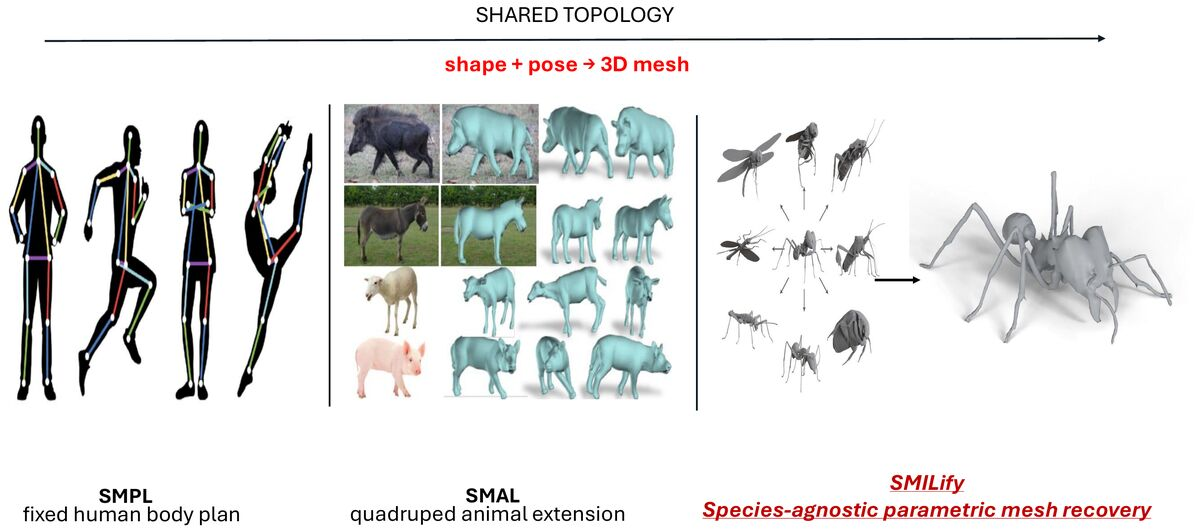
\includegraphics[width=0.62\linewidth]{figures/fig_model_lineage.jpg}
\caption[Lineage of parametric models]{Lineage of body-plan-agnostic
parametric models: a fixed human topology (SMPL), a shared quadruped rig
learned from toy figurines (SMAL), and SMILify, which fits an arbitrary rigged
template to scan-derived meshes of any body plan.}
\label{fig:lineage}
\end{figure}

The internship was supervised by Dr.\ Fabian Plum, postdoctoral researcher at
IAS-7 and author of scAnt~\cite{scant}, replicAnt~\cite{replicant},
OmniTrax~\cite{omnitrax} and SMILify, and ran on site from 1 July to
25 September 2026. Two aspects of that arrangement shaped the work. First,
the assignments of the brief were an initial hypothesis rather than a fixed
specification, so redirecting the work when the evidence required it was
the correct response. Second, development took place on a live shared
repository under pull-request review, with the supervisor running related
experiments on adjacent branches; several results were revised following that
review, and the practice of fixing the success criterion of an experiment
before running it follows directly from it. The shared allocation on the JSC
machines could not absorb the full compute demand, so the heaviest experiments
also ran on an RWTH allocation with H100 GPUs (Section~\ref{sec:setup}).
